\documentclass[12pt, a5paper, parskip=half-]{scrartcl}
\usepackage{tikz}
\usetikzlibrary{arrows.meta}
\usetikzlibrary{shapes}
\usetikzlibrary{calc}
\usetikzlibrary{decorations.pathmorphing}

\usepackage[skins]{tcolorbox}

\usepackage[bmargin=2.5cm, lmargin=1.7cm, rmargin=1.7cm, tmargin=1.5cm]{geometry}

% Adjust spacing before and after section headings
\RedeclareSectionCommand[
  runin=false,
  beforeskip=0.5\baselineskip,
  afterskip=-0.25\baselineskip
]{section}

\RedeclareSectionCommand[
  runin=false,
  beforeskip=0.5\baselineskip,
  afterskip=-0.25\baselineskip
]{subsection}

\RedeclareSectionCommand[
  runin=false,
  beforeskip=0.5\baselineskip,
  afterskip=-0.25\baselineskip
]{subsubsection}

%\usepackage[pass]{geometry}
\usepackage{fontspec} % Use system fonts.  Not compatible with pdflatex. Use XeLaTeX instead!
\usepackage{cinzel}
 \newfontfamily\displayfont{Cinzel}
\setkomafont{section}{\large\cinzel\bfseries}
\setkomafont{subsection}{\cinzel\bfseries}
\setkomafont{subsubsection}{\small\cinzel\bfseries}


\usepackage{enumitem} % Adjust formatting of description environment items
\usepackage{calc}

\usepackage{multicol} % Format list of playtesters in two columns

\usepackage[type={CC}, version={4.0}, modifier={by}]{doclicense} % Add text and icons for creative commons license

\usepackage{contour}

%dice mini-diagrams

\tikzset{die1/.pic={
    	\node[draw, very thick,minimum size=1em, rounded corners=1mm] {};
    	\node[draw, fill=black, circle, inner sep=0.65pt] {};
	}
}

\tikzset{die2/.pic={
    	\node[draw, very thick,minimum size=1em, rounded corners=1mm] {};
    	\node[draw, fill=black, circle, inner sep=0.65pt] at (0.1, 0.1) {};
    	\node[draw, fill=black, circle, inner sep=0.65pt] at (-0.1,  -0.1) {};
	}
}

\tikzset{die3/.pic={
    	\node[draw, very thick,minimum size=1em, rounded corners=1mm] {};
    	\node[draw, fill=black, circle, inner sep=0.65pt] {};
    	\node[draw, fill=black, circle, inner sep=0.65pt] at (0.1, 0.1) {};
    	\node[draw, fill=black, circle, inner sep=0.65pt] at (-0.1,  -0.1) {};
	}
}

\tikzset{die4/.pic={
    	\node[draw, very thick,minimum size=1em, rounded corners=1mm] {};
    	\node[draw, fill=black, circle, inner sep=0.65pt] at (0.1, 0.1) {};
    	\node[draw, fill=black, circle, inner sep=0.65pt] at (0.1, -0.1) {};
    	\node[draw, fill=black, circle, inner sep=0.65pt] at (-0.1, 0.1) {};
    	\node[draw, fill=black, circle, inner sep=0.65pt] at (-0.1,  -0.1) {};
	}
}

\tikzset{die5/.pic={
    	\node[draw, very thick,minimum size=1em, rounded corners=1mm] {};
    	\node[draw, fill=black, circle, inner sep=0.65pt] {};
    	\node[draw, fill=black, circle, inner sep=0.65pt] at (0.1, 0.1) {};
    	\node[draw, fill=black, circle, inner sep=0.65pt] at (-0.1,  -0.1) {};
    	\node[draw, fill=black, circle, inner sep=0.65pt] at (0.1, -0.1) {};
    	\node[draw, fill=black, circle, inner sep=0.65pt] at (-0.1,  0.1) {};

	}
}

\tikzset{die6/.pic={
    	\node[draw, very thick,minimum size=1em, rounded corners=1mm] {};
     \node[draw, fill=black, circle, inner sep=0.65pt] at (0.1, 0.1) {};
    	\node[draw, fill=black, circle, inner sep=0.65pt] at (-0.1,  -0.1) {};
    	\node[draw, fill=black, circle, inner sep=0.65pt] at (0.1, -0.1) {};
    	\node[draw, fill=black, circle, inner sep=0.65pt] at (-0.1,  0.1) {};
    	\node[draw, fill=black, circle, inner sep=0.65pt] at (-0.1,  0) {};
    	\node[draw, fill=black, circle, inner sep=0.65pt] at (0.1, 0) {};

	}
}

%fancy page numbers
\renewcommand{\pagemark}{
	\begin{tikzpicture}[scale=0.2]
		\node[draw, star, star points = 9, star point ratio = 0.5, rounded corners=1.25mm, minimum size=3.0cm, semithick, rotate=27.5, transform shape] (a) at (0,0) {};
		\foreach \i in {0,1,2,3,4,5,6,7,8}
			\node[draw, circle, semithick, transform shape, minimum size=0.45cm] (a\i) at (40*\i + 1:2.75cm) {};

		\node (b) at (0,0) {\arabic{page}};
%		\node at (0,6.5) {}; % Add some white space at the top to make the image render a bit lower.
	\end{tikzpicture}
}

\usepackage{fancyhdr}
\fancypagestyle{titleheader}{%
	\fancyhead{}
	\fancyfoot{}
	\renewcommand{\headrulewidth}{0pt}
	\chead{\footnotesize Draft Version 0.3}
}
%
\fancypagestyle{colortitleheader}{%
	\fancyhead{}
	\fancyfoot{}
	\renewcommand{\headrulewidth}{0pt}
	\chead{\footnotesize \textcolor{lightgray}{Draft Version 0.3}}
}

%
\fancypagestyle{bodyheaderfooter}{%
	\fancyhead{}
	\fancyfoot{}
	\renewcommand{\headrulewidth}{0pt}
	\chead{\footnotesize Draft Version 0.3}
	\cfoot{\pagemark}
}

\pagestyle{bodyheaderfooter}

\usepackage{pdfpages}

\usepackage[hidelinks]{hyperref} % This should usually be the last package loaded before \begin{document}
\usepackage[xspace]{ellipsis} % This package is one of the few packages that must be loaded after hyperref
\begin{document}

%%=========================================
%% Color Title Page
%\begin{titlepage}
%		\enlargethispage{3.5\baselineskip} % Move the bottom line (author and date) down a bit
%
%		\begin{tikzpicture}[remember picture, overlay]
%		\draw[fill stretch image=Images/black_marble_texture_vertical.png]  (current page.south west) rectangle (current page.north east);
%%		\draw[fill=black]  (current page.south west) rectangle (current page.north east);
%%
%		\end{tikzpicture}
%
%         \setmainfont{Cinzel Decorative}
%	    \centering{
%			{\fontsize{60}{72}\selectfont \textcolor{violet!75}{pROpHecY}}
%		}
%
%		\setmainfont{URWClassico}
%		\vspace{5mm}
%		\centering{\Large{\contour{black}{\textcolor{lightgray}{A tabletop roleplaying game}} \\ \smallskip \contour{black}{\textcolor{lightgray}{about fate and destiny}}}}
%
%		\vfill
%
%		
\includegraphics[scale=3.81]{Images/comet_diagram_violet.pdf}
%
%		\vfill
%		
%		\Large{\contour{black}{\textcolor{lightgray}{Michael Purcell}}}
%
%\end{titlepage}
%%
%%=========================================
%
%
%%=========================================
%% BW Title Page
%\begin{titlepage}
%	\thispagestyle{titleheader}
%		\enlargethispage{3.5\baselineskip} % Move the bottom line (author and date) down a bit
%		
%         \setmainfont{Cinzel Decorative}
%	    \centering{
%			{\fontsize{60}{72}\selectfont
%			{\textcolor{black}{pROpHecY}}}
%		}
%
%		\setmainfont{URWClassico}
%		\vspace{5mm}
%		\centering{\Large{{\textcolor{black}{A tabletop roleplaying game \\ \smallskip about fate and destiny}}}}
%
%		\vfill
%
%		
\includegraphics[scale=3.81]{Images/comet_diagram.pdf}
%
%		\vfill
%		
%		\Large{{\textcolor{black}{Michael Purcell}}}\\
%\end{titlepage}
%
%%=========================================

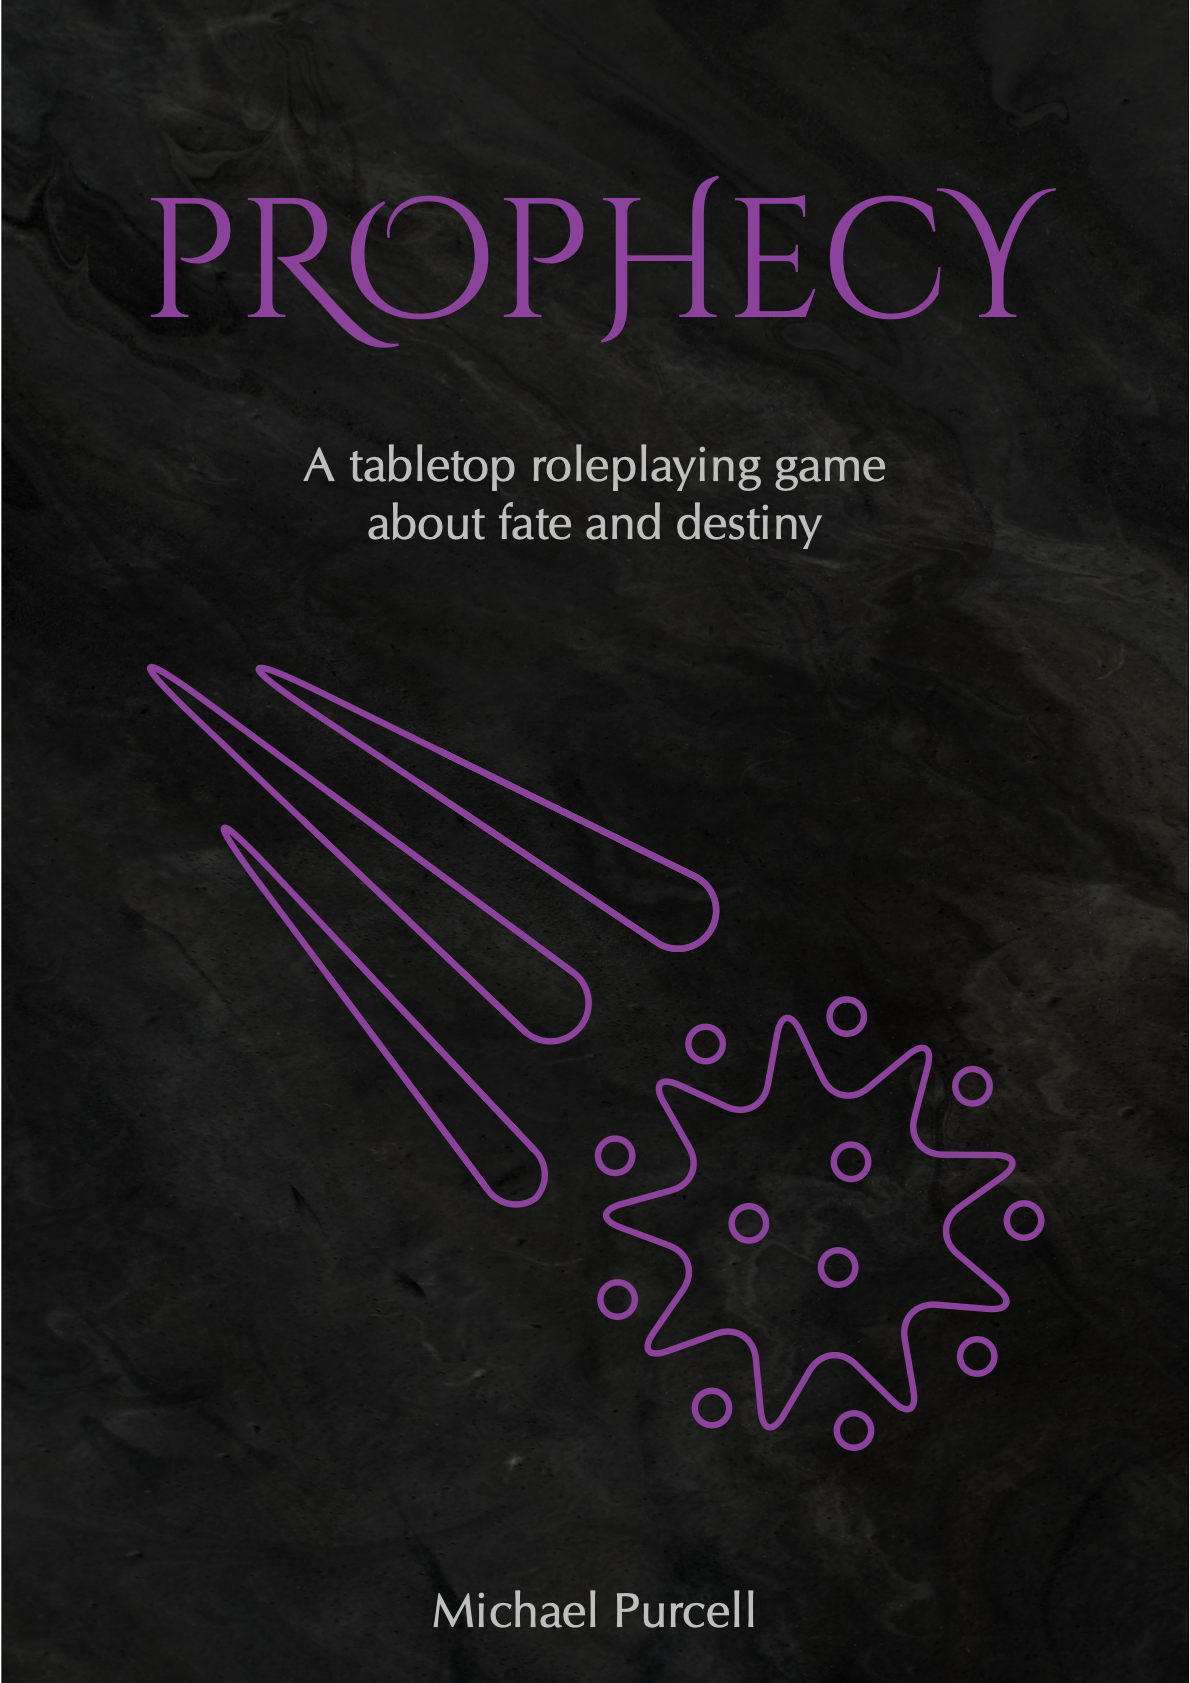
\includepdf{prophecy_colour_cover}

\setmainfont{URWClassico}
\normalsize

\RedeclareSectionCommand[
  runin=false,
  beforeskip=0.5\baselineskip,
  afterskip=-0.25\baselineskip
]{section}

\center

\setcounter{page}{1}
\section*{\huge \phantom{a} \hfill The Dragon Wakes \hfill \phantom{a}} \label{section:the-dragon-wakes}
\vfill
Long ago, in the first age of men,\\
the world was filled with wonders. \\
The people thought themselves safe \\
from the fury of the natural world.

\smallskip

Then She came.

\smallskip

The Dragon emerged from the sea\\and laid waste to the land.\\
Only the grandest works\\of those once great civilisations\\remain to mark their passage.

\smallskip

Or so the story goes.

\smallskip

Most scholars believe that\\the Dragon is a myth\\and that the Ancients were\\responsible for their own demise.
%Others believe that while\\the Dragon was real,\\She must have died long ago.

\smallskip

They are mistaken. 

\smallskip

%After one thousand years of slumber,\\
%the Dragon wakes. \\
The earth shakes as She begins to stir.\\
The oceans froth and swell as\\She shakes off the last vestiges of sleep.\\
Now we face the same fate\\as that which befell our forebears.
\vfill

\newpage

\RedeclareSectionCommand[
  runin=false,
  beforeskip=0.5\baselineskip,
  afterskip=-0.25\baselineskip
]{section}

\raggedright
\section*{Introduction} \label{section:introduction}
Prophecy is a GM-less roleplaying game for three to six people that can be played in under three hours.
During the game, the players receive a prophecy that describes an impending catastrophe for some fictional world and tell a story about characters whose lives will be affected by that catastrophe. 

The players first decide the basic outline of the story,describing events that are fated to occur.  They then fill in the details of the story, describing how the characters try to shape their destiny.

Throughout these rules, a variety of common words are used as technical terms to describe how the game is played.
These terms will be \emph{italicised} when they are first introduced.
References to sections of the rules will be written in the same font as the \hyperref[section:introduction]{\cinzel \small Section Headings}.

\subsection*{Materials} \label{subsection:materials}
To play the game the players will need a few materials that they will use to take notes and determine outcomes. They will need:
\begin{description}[labelindent=0.25cm, leftmargin=\widthof{\hspace{0.25cm}\textbullet\space}, font=\normalfont\textbullet\bfseries\space]
	\item[Index Cards:] Approximately fifty index cards should be placed within easy reach of all players. 
	\item[Sticky Notes:] Approximately one hundred sticky notes should be placed within easy reach of all players.
	\item[Butcher Paper:] One large sheet of butcher paper should be placed in the middle of the play area.  A whiteboard can be used instead if desired. This is the \emph{story board}. 
	\item[Markers:] Each player should have a marker to write on the index cards, sticky notes, and story board.
	\item[Dice:] Approximately twelve six-sided dice should be placed within easy reach of all players. 
\end{description}

\newpage

\subsection*{Collaborative Storytelling} \label{subsection:collaborative-storytelling}
Prophecy is a storytelling game.
As such, the players' ultimate goal in the game should be to tell an interesting story.
The rules of the game are designed to help the players do so.
If at any point the players need to choose between following the rules or telling a good story, they should choose the latter.

Prophecy is also a collaborative game.
Collaboration implies shared ownership.
As such, the players should be equal partners in the playing of the game.
No player should ever try to unilaterally dictate what happens in the story and no player should ever feel like their contributions have been ignored or overruled by another player.

\subsection*{Safety Tools} \label{subsection:safety-tools}
Because stories can provoke strong emotional responses, the players should be sensitive to one another's feelings during the game.
They should avoid, or retroactively remove, any content that makes any of the players uncomfortable.

It can be difficult, however,  to identify such content. 
So, the players should establish some ground rules about what should be excluded before the game begins. 
They should also establish a way to indicate that something in the story has made someone uncomfortable and should be removed or replaced.

Players who identify problematic content do not need to explain themselves.
Because the other players may not know what the problem is, the player who identified the issue should suggest a satisfactory alternative.

\newpage

\section*{Mechanics}  \label{section:mechanics}
\emph{Mechanics} are the systems that govern how the players interact with the game.
They provide a way for the players to describe a fictional world, compose a story set in that world, and determine how that story plays out.

\subsection*{Objects and Aspects} \label{subsection:objects-and-aspects}
An \emph{object} is a person, place, or thing that appears in the story.
An \emph{aspect} is a word or short phrase that describes something noteworthy about an object.
An aspect that describes an object is \emph{attached} to that object.

The players should use index cards to represent objects and sticky notes to represent aspects. 
If an aspect is attached to an object, then the players should stick the note for that aspect to the card for that object.

\subsubsection*{Characters} \label{subsubsection:characters}
A \emph{character} is a person who appears in the story and who  is controlled by a single player throughout the game. 
Note that, within the framework of the game, characters are objects.
So, aspects can be attached to characters.
An aspect that is attached to a character is a \emph{character~aspect}.

\subsubsection*{Environment} \label{subsubsectioon:environment}
Any object that is not a character is a part of the \emph{environment}.
Note that, within the framework of the game, most of the people who appear in the game are not characters.
They are part of the environment. 
An aspect that is attached to any part of the environment is an \emph{environment~aspect}.

\newpage

\subsection*{Matching Aspects} \label{subsection:matching-aspects}
A pair of \emph{matching aspects} is a set of two aspects, one character~aspect and one environment~aspect, that together allow the characters to manipulate a scene to their advantage.

There are no definitive criteria for what constitutes a pair of matching aspects. 
For each candidate pair, the players should discuss how the interaction between the two aspects would make it easier for the characters to accomplish their objective in the scene. If the players agree that the pair would do so, then they are matching aspects. Otherwise, they are not.

\subsubsection*{Example} \label{example:matching-aspects}
Suppose that the players are telling a story in which the characters are trying to deal with the prophecy described in \hyperref[subsection:the-tachyonic-antitelephone]{\cinzel \small The Tachyonic Antitelephone}. 

One of the characters, Ruth,  is trying to infiltrate a government lab where dangerous time-travel experiments are being conducted.  There is a guard posted at the main entrance.

Several aspects are attached to Ruth, including:\vspace{-1.75ex}
\begin{multicols}{2}
\begin{itemize}[noitemsep,nolistsep,  leftmargin=0.68cm]
  \item DARPA research scientist
  \item Independently wealthy
  \item Acerbic wit
  \item Brilliant physicist
\end{itemize}
\end{multicols}
\vspace{-2ex}
Several aspects are attached to the guard, including:\vspace{-1.75ex}
\begin{multicols}{2}
\begin{itemize}[noitemsep,nolistsep,  leftmargin=0.68cm]
	\item Overworked
	\item Underpaid
\end{itemize}
\end{multicols}
\vspace{-2ex}
The players identify a candidate pair of aspects:
\begin{itemize}[leftmargin=0.68cm, noitemsep,topsep=-1ex]
	\item Independently wealthy / Underpaid.
\end{itemize}
\vspace{1ex}

After some discussion, the players agree that together these two aspects suggest that Ruth might be able to bribe the guard to let her into the lab.  So, they are matching aspects.

\newpage

\subsection*{Scenes} \label{subsection:scenes}
A \emph{scene} is a part of the story that describes the events that happen at a single time and place.
Every scene has the following components:
\begin{description}[labelindent=0.25cm, leftmargin=\widthof{\hspace{0.25cm}\textbullet\space}, font=\normalfont\textbullet\bfseries\space]
  \item[Setting:]
  The time and place at which the scene occurs and the objects and aspects that appear in the scene.
  \item[Objective:]
    A description of what the characters are trying to accomplish during the scene.
  \item[Difficulty Rating:]
    A number that describes how difficult it is for the characters to accomplish the scene's objective.
  \item[Outcome:]
    A description of whether the characters accomplish the scene's objective. If so, then the outcome is a \emph{success}.  If not, then the outcome is a \emph{failure}.
  \item[Precursors:]
    Other scenes which, if resolved successfully, make it easier for the characters to accomplish the scene's objective.
    A scene is the \emph{parent} of its precursors.
\end{description} 

\bigskip

The players should use ovals drawn on the story board to represent scenes and lines to represent relationships between scenes.
The players should draw lines connecting each scene with its precursors.

\newpage

\subsubsection*{Sketching Scenes} \label{subsubsection:sketching-scenes}
The players \emph{sketch} scenes when they \hyperref[subsection:write-an-outline]{\cinzel \small Write an Outline}. 
To sketch a scene the players will establish the setting, define the objective, and assign the difficulty rating for the scene.

When they sketch a scene, the players should draw an oval on the story board to represent the scene, and label the oval with the scene's objective and difficulty rating.
If the scene is a precursor to an existing scene, then the players should draw a line on the story board connecting the ovals that represent the two scenes.

\subsubsection*{Performing Scenes} \label{subsubsection:performing-scenes}
The players \emph{perform} scenes when they \hyperref[subsection:tell-the-story]{\cinzel \small Tell the Story}.
To perform a scene the players will describe what happens during the scene, determine the outcome of the scene, and describe the consequences of the characters' actions.

Before they make a check to determine the outcome of a scene, the players should roleplay interactions between the characters and the objects that populate the scene.

After the outcome of a scene has been determined, the players should describe the characters' actions in the scene and how they led to the specified outcome.
This description should be informed by the pairs of matching aspects that the characters attempted to use to manipulate the scene to their advantage.

After performing each scene, the players should cross out the oval representing that scene on the story board. If the scene was resolved successfully, the players should place a die on the oval that represents that scene's parent.
\newpage

\subsection*{Checks} \label{subsection:checks}
The players make a \emph{check} to determine the outcome of each scene.
To make a check, the players will:
\begin{description}[labelindent=0.25cm, leftmargin=\widthof{\hspace{0.25cm}\textbullet\space}, font=\normalfont\textbullet\bfseries\space]%[leftmargin=0pt]
\item[Assemble a Dice Pool:]
     A dice pool is made up of one or more six-sided dice.
     One die is added to the pool for each pair of matching aspects that characters could use to manipulate the scene to their advantage.
     In addition, one die is added to the pool for each of the current scene's precursors that was resolved successfully.
 \item[Roll the Dice:]
     The dice are exploding dice.
     That is, for every die that yields \tikz[baseline=-0.35em]{\pic {die6};} another die is added to the pool.
\item[Compute the Result:]
     Any die that yields \tikz[baseline=-0.35em]{\pic {die1};}, \tikz[baseline=-0.35em]{\pic {die2};}, or \tikz[baseline=-0.35em]{\pic {die3};} is a \emph{miss}.
     Any die that yields \tikz[baseline=-0.35em]{\pic {die4};}, \tikz[baseline=-0.35em]{\pic {die5};}, or \tikz[baseline=-0.35em]{\pic {die6};} is a \emph{hit}.
     The \emph{result} of a roll is the total number of hits.
\item[Determine the Outcome:]
     If the result of the players' roll meets or exceeds the scene's difficulty rating, then the outcome is a success,
     otherwise it is a failure.
 \end{description}
\bigskip
Optionally, the players can keep track of the reason that each die was added to the pool.  Hits and misses can then be interpreted individually as well as collectively.  The players can incorporate these nuances when they describe how the  characters' actions led to the outcome of each scene.
\newpage

\subsubsection*{Example} \label{example:checks}
Suppose that the players are making a check to determine the outcome of a scene where the characters are trying to deal with the prophecy described in \hyperref[subsection:project-spaceguard]{\cinzel \small Project Spaceguard}.

The objective of the scene is:
\begin{itemize}[leftmargin=\widthof{\hspace{0.25cm}\textbullet\space}, noitemsep,topsep=-1ex]
\item Smuggle the children aboard a colony ship.
\end{itemize}
\vspace{1ex}
The difficulty rating of the scene is (4). 

The players identify three pairs of matching aspects that the characters can use to manipulate the scene to their advantage:
\begin{itemize}[leftmargin=\widthof{\hspace{0.25cm}\textbullet\space}, noitemsep, topsep=-1ex]
\item Defence contractor / Built by the lowest bidder,
\item Armed and dangerous / I'm a doctor not a soldier,
\item Expert hacker / It's a UNIX system!
\end{itemize}
\vspace{1ex}
Two of the scene's precursors were resolved successfully. The objectives of those scenes were:
\begin{itemize}[leftmargin=\widthof{\hspace{0.25cm}\textbullet\space}, nosep, topsep=-1ex]
\item Befriend one of the flight controllers,
\item Steal a set of crew uniforms.
\end{itemize}
\vspace{1ex}
So, the dice pool initially consists of five dice.

When rolled, these dice yield \tikz[baseline=-0.35em]{\pic {die3};}, \tikz[baseline=-0.35em]{\pic {die6};}, \tikz[baseline=-0.35em]{\pic {die5};}, \tikz[baseline=-0.35em]{\pic {die1};},  \tikz[baseline=-0.35em]{\pic {die6};}.% the values {3, 6, 5, 1, 6}. %
\ Because two dice yielded \tikz[baseline=-0.35em]{\pic {die6};}, two dice are added to the pool.
When rolled, these dice yield \tikz[baseline=-0.35em]{\pic {die2};}, \tikz[baseline=-0.35em]{\pic {die6};}.%{2,6}.
\ Because one die yielded \tikz[baseline=-0.35em]{\pic {die6};}, another die is added to the pool.
When rolled, this die yields \tikz[baseline=-0.35em]{\pic {die4};}.

Altogether, the final roll yields \tikz[baseline=-0.35em]{\pic {die3};}, \tikz[baseline=-0.35em]{\pic {die6};}, \tikz[baseline=-0.35em]{\pic {die5};}, \tikz[baseline=-0.35em]{\pic {die1};}, \tikz[baseline=-0.35em]{\pic {die6};}, \tikz[baseline=-0.35em]{\pic {die2};}, \tikz[baseline=-0.35em]{\pic {die6};}, \tikz[baseline=-0.35em]{\pic {die4};}.%{3, 6, 5, 1, 6, 2, 6, 4}.

Because five dice yielded \tikz[baseline=-0.35em]{\pic {die4};},  \tikz[baseline=-0.35em]{\pic {die5};}, or \tikz[baseline=-0.35em]{\pic {die6};}, the result of this roll is five hits.
As this exceeds the difficulty rating of the scene, the outcome of the check is a success.
The characters are able to smuggle the children aboard a colony ship.

\newpage

\section*{Gameplay} \label{section:gameplay}
The game is divided into four phases.
The first three phases are about fate.
The players will:
\begin{description}[labelindent=0.25cm, leftmargin=\widthof{\hspace{0.25cm}\textbullet\space}, font=\normalfont\textbullet\bfseries\cinzel\small\space]
  \item[{\hyperref[subsection:receive-a-prophecy]{Receive a Prophecy}:}] The prophecy describes an impending catastrophe for some fictional world.
  \item[{\hyperref[subsection:create-characters]{Create Characters}:}] The characters inhabit the fictional world that the players create.
  \item[{\hyperref[subsection:write-an-outline]{Write an Outline}:}] The outline describes the story that the players will tell about the characters.
\end{description}

The fourth phase is about destiny.
The players will:
\begin{description}[labelindent=0.25cm, leftmargin=\widthof{\hspace{0.25cm}\textbullet\space}, font=\normalfont\textbullet\bfseries\cinzel\small\space]
	\item[{\hyperref[subsection:tell-the-story]{Tell the Story}:}] The story describes the characters' adventures as they try to deal with the catastrophe.
\end{description}

\bigskip

The game should be tightly focused on the question of how the characters will try to deal with the catastrophe.
The story should consist of no more than eight scenes and each scene should be performed in less than ten minutes. 

\subsection*{Receive a Prophecy} \label{subsection:receive-a-prophecy}
During this phase, the players receive a prophecy that describes an impending catastrophe that is destined to wreak havoc within a fictional world.

The players should describe the world in which the story is set and the nature of the catastrophe.
The catastrophe should be inevitable and significant, with pervasive and disruptive effects.

Several pre-written  prophecies are provided as \hyperref[section:modules]{\cinzel \small Modules}.

\newpage

\subsection*{Create Characters} \label{subsection:create-characters}
During this phase, each player will create a character.
Later in the game, the players will assume the identities of these characters when they perform scenes.

Each player should first choose a name for their character and then attach one aspect from each of the following categories to their character:
\begin{description}[labelindent=0.25cm, leftmargin=\widthof{\hspace{0.25cm}\textbullet\space}, font=\normalfont\textbullet\bfseries\space]
   \item[Occupation:]
     An aspect that describes the character's profession, hobbies, or other interests.
   \item[Physical Characteristic:]
     An aspect that describes the character's body or mind.
   \item[Psychological Characteristic:]
     An aspect that describes the character's personality.
   \item[Relationship:]
     An aspect that describes the character's connection with another person.
   \item[Affiliation:]
     An aspect that describes the character's connection with an organisation.
\end{description}

\bigskip

During the game additional aspects can be attached to a character and existing aspects can be modified to reflect how a character changes in response to the events that occur as the players \hyperref[subsection:tell-the-story]{\cinzel \small Tell the Story}.

\newpage

\subsection*{Write an Outline} \label{subsection:write-an-outline}
During this phase, the players will write an \emph{outline} that describes how the characters will try to deal with the catastrophe.
The outline describes a collection of scenes that are arranged in a hierarchical tree-like structure.

The players should first sketch a scene called the \emph{finale}.
Then, the players should sketch additional scenes that describe the events that will lead to the finale.

\subsubsection*{Sketch the Finale} \label{subsubsection:sketch-the-finale}
The objective of the finale should describe how the characters intend to deal with the catastrophe.
The difficulty rating of the finale is always (5).
The finale will be the last scene that the players perform when they \hyperref[subsection:tell-the-story]{\cinzel \small Tell the Story}.

\subsubsection*{Sketch Additional Scenes} \label{subsubsection:sketch-additional-scenes}
Each additional scene must be a precursor of an existing scene.
The difficulty rating of the new scene is always one less than that of the existing scene and must be greater than zero.

The objective for each new scene should be chosen such that, if the scene is resolved successfully, then it will be easier to accomplish the objective of its parent. One way of doing so is to ensure that accomplishing the objective of each new scene will provide the characters with either the motive, means, or opportunity to accomplish the objective of an existing scene.

\newpage

\subsubsection*{Example} \label{example:write-an-outline}
Suppose that the players are writing an outline for a story about how the characters might try to deal with the prophecy described in \hyperref[section:the-dragon-wakes]{\cinzel \small The Dragon Wakes}.  They decide that the finale will be an epic battle with the Dragon and that the other scenes will be about how the characters prepare for that confrontation.

The outline that the players create might look something like the following diagram:
\smallskip
\begin{center}
\begin{tikzpicture}[every path/.style={very thick}, every node/.style={draw, rounded corners=2mm, minimum width=3cm}]
\node[text width=4cm, align=center] (s1) at (0,0) {(5) Defeat the Dragon in Battle};
\node[text width=4cm, align=center]   (s11) at (-3,2) {(4) Recruit Allies to Fight the Dragon};
\node[text width=4cm, align=center]  (s12) at (0,4) {(4) Lure the Dragon into a Trap};
\node[text width=4cm, align=center]  (s13) at (3,2) {(4) Discover the Dragon's Weakness};
\node[text width=4cm, align=center]  (s121) at (-3,6) {(3) Figure Out What the Dragon Wants};
\node[text width=4cm, align=center] (s122) at (0,8) {(3) Locate the Dragon's Lair};
\node[text width=4cm, align=center] (s131) at (3,6) {(3) Find Lost Stories About the Dragon};

\draw[very thick, -{Latex}] (s11) -- (s1);
\draw[very thick, -{Latex}] (s12) -- (s1);
\draw[very thick, -{Latex}] (s13) -- (s1);
\draw[very thick,-{Latex}] (s121) -- (s12);
\draw[very thick,-{Latex}] (s122) -- (s12);
\draw[very thick,-{Latex}] (s131) -- (s13);
\end{tikzpicture}
\end{center}
\smallskip
The numbers in parentheses indicate the difficulty rating of the corresponding scenes. 

\newpage

\subsection*{Tell the Story} \label{subsection:tell-the-story}
During this phase, the players will tell the story of the characters' adventures as they try to enact their plan to deal with the catastrophe.
The players will perform scenes to discover how the story unfolds and how the characters are affected.

The players will perform the scenes described in the outline.
A scene cannot be performed until after all of its precursors have been performed.
Other than this restriction, however, the scenes can be performed in any order.

\subsubsection*{Perform the Finale} \label{subsubsection:perform-the-finale}
The finale will be the last scene that the players perform and the outcome of the finale will determine if the characters are able to successfully execute their plan to deal with the catastrophe.
So, the consequences of the characters' actions in this scene are particularly important.

As with any scene, the players should describe the characters' actions, how they led to the specified outcome, and the immediate consequences of those actions.
In the finale, however, they should also describe the long-term effects that the catastrophe has on the world.



\newpage

\section*{The Moderator} \label{section:the-moderator}
Optionally, one of the players can assume the role of \emph{moderator}. The moderator's job is to help the other players play the game. This assistance can take a variety of forms: answering questions about the rules, managing logistics, or ensuring that everyone agrees about various details of the story.

\subsubsection*{Asking Questions} \label{subsubsection:asking-questions}
The moderator should encourage the other players to tell an interesting story by asking them questions.  If the moderator is curious about something in the story and wants to learn more, then they should ask for more information.  Similarly, if the moderator is confused then they should ask for clarification.

Importantly, however, the moderator's role is not prescriptive.  The moderator should not narrate any part of the story. The moderator can make suggestions or present alternatives, but ultimately the other players should decide what happens.

\subsubsection*{Keeping Time} \label{subsubsection:keeeping-time}
The moderator should act as a timekeeper. 
The moderator should start a timer when the other players begin to perform a scene.
At the end of ten minutes, or if the other the other players are starting to struggle to make contributions, the moderator should suggest that it may be time to move on.

\newpage

\section*{Modules} \label{section:modules}
The first thing that the players do is \hyperref[subsection:receive-a-prophecy]{\cinzel \small Receive a Prophecy}.  \\
This is the inciting incident for everything that happens in the story.
%It's important!
By describing the catastrophe, the players establish the foundation on which the rest the game will be built.

A \emph{module} is a pre-written prophecy designed to help the players get started.
Each module describes a catastrophe as it might be presented to characters who are hearing the prophecy for the first time.  The players should read the module aloud and populate the world that it implies with objects and aspects.

\subsection*{The Tachyonic Antitelephone} \label{subsection:the-tachyonic-antitelephone}
I am, well \ldots I'm you.  That is, I was. Or, you will be.  Or, something like that. Anyway, I'm afraid that I've got some bad news. Really bad. You see, it turns out that the work that you did for DARPA last year was used to create something that we used to think impossible.
They built a time machine. 

Fortunately, it's pretty limited.  It can only send messages back in time, and then only to times after they turned it on.  That's why I'm talking to you now instead of earlier when it might have done some good.

Unfortunately, it turns out that messing around with time is a bad idea.
Really bad. It didn't take long before strange things started to happen.
Then the Time Eaters came.

It's too late for us. 
Maybe, though, its not too late for you.
If nothing else, you might be able to pass this message along in turn when you get here. 
Eventually, one of us is sure to figure a way out of this mess.
Right?

%\subsection*{Return of the Dragon} \label{subsection:return-of-the-dragon}
%Long ago, in the first age of men, the world was filled with wonders. 
%The people of that time thought themselves safe from the fury of the natural world.
%Then She came.
%The great Dragon emerged from the sea and laid waste to the land.
%Only the grandest works of those once great civilisations remain to mark their passage.
%
%Or so the story goes.
%Most scholars believe that the Dragon is a myth and that the Ancients were somehow responsible for their own demise.
%Others believe that while the Dragon was real, She must surely have died long ago.
%They are mistaken. 
%
%After one thousand years of slumber, the Dragon wakes. 
%The earth shakes as She begins to stir.
%The oceans froth and swell as She shakes off the last vestiges of sleep.
%Now we face the same fate as that which befell our forebears.

\newpage

\subsection*{Project Spaceguard} \label{subsection:project-spaceguard}
My fellow Americans, it is with a heavy heart that I come to you tonight. 
As you are doubtless aware, last year the initial survey conducted as a part of Project Spaceguard discovered a large Near Earth Object that was projected to collide with the Earth later this month.
Ever since, the primary focus of this administration has been to prevent that from occurring. Earlier this evening, the director of Project Spaceguard informed me that we have failed.

Now, we must shift our focus from preventing a collision to surviving its aftermath.
Effective immediately, I am declaring a nationwide state of emergency. 
National Guard units will be activated and deployed in support of local law enforcement. 

Going forward, the Federal Emergency Management Agency will be leading our response.
I'll turn the microphone over to the director of that agency now and he can provide details about what you can expect.
Goodnight and Godspeed.


\subsection*{She's Having a Baby} \label{subsection:shes-having-a-baby}
Congratulations! It looks like you're at about eight weeks now.
Everything looks great, both mum and bub are doing fine. 
So, we'll plan on seeing you again in about four weeks.

While you're here I should tell you about the course that the hospital offers for new parents.
It's a great way to learn about what to expect and a chance talk to other new parents about the whole experience. 
The teachers are all former maternity ward nurses, and they really do a great job.

I know that this can be overwhelming.
If you have any concerns, please give us a call at any time. 

\newpage

\subsection*{The Deluge \setmainfont{URWClassico}- From The King James Version of the Bible} \label{subsection:the-deluge}
I will destroy man whom I have created from the face of the earth; both man, and beast, and the creeping thing, and the fowls of the air; for it repenteth me that I have made them.\\ 
\vspace{0.5ex}\hspace{8cm} - Genesis 6:7

And, behold, I, even I, do bring a flood of waters upon the earth, to destroy all flesh, wherein is the breath of life, from under heaven; and every thing that is in the earth shall die. \\
\vspace{0.5ex}\hspace{8cm} - Genesis 6:17

For yet seven days, and I will cause it to rain upon the earth forty days and forty nights; and every living substance that I have made will I destroy from off the face of the earth.\\
\vspace{0.5ex}\hspace{8cm} - Genesis 7:4

\subsection*{Unsafe at Any Speed \setmainfont{URWClassico} - Submitted by Paul Murray} \label{subsection:unsafe-at-any-speed}
You know what this means don't you?
That crackpot down in R\&D was right. 
Every Faraday Byron that we've sold in the past two years is a ticking time bomb.
The first ones off the assembly line are going to start failing soon.
After that, every week will be worse than the one before.

We're not going to be able to keep this quiet for long.
Soon, even your pet politicians are going to have to do something.
What then?
Eventually they're going to figure out that we knew this might happen.
I bet it takes them less than a month.

Someone is going down for this, and it's not going to be me.
I'm leaving!
Maybe I'll go somewhere warm. 
Somewhere with white-sand beaches, palm trees,  and no extradition treaty.

\newpage

%\subsection*{The Tachyonic Antitelephone} \label{subsection:the-tachyonic-antitelephone}
%Is this thing on? I hope so.  If you're hearing this, then I imagine you must be asking yourself quite a few questions right now. I'm afraid that they'll have to wait; I don't have much time. Hah!
%
%I am, well \ldots I'm you.  That is, I was. Or, you will be.  Or, something like that. Anyway, I'm afraid that I've got some bad news. Really bad. You see, it turns out that the work that you did for the government last year was used to create something that we used to think impossible.
%
%They've built a time machine.  Fortunately, it's pretty limited.  It can only send messages back in time, and then only to times after they turned it on.  That's why I'm talking to you now instead of earlier when it might have done some good.
%
%Unfortunately, it turns out that messing around with time is a bad idea. Really bad. It didn't take long before strange things started to happen. Then the time eaters came.  Needless to say, they aren't here to say hello and welcome us to the neighbourhood. 
%Rather, they seem to be some kind of pangalactic exterminators and they are very good at their job.
%
%It won't be long before the time eaters finish their work.
%They've already killed ninety percent of the population and show no signs of stopping.
%I've only managed to escape for this long because the fools who created this thing brought me in to help them fix the mess that they've made.  
%
%Alas, It's too late for us. Maybe, though, its not too late for you.
%If nothing else, you might be able to pass this message along in turn when you get here. 
%Eventually, one of us is sure to figure a way out of this mess.
%Right?
%
%\newpage

\subsection*{Dead Man's Switch  \setmainfont{URWClassico} - Submitted by Brett Witty} \label{subsection:dead-mans-switch}
If you're hearing this, I am dead.
But you probably already know that.
I haven't contacted my fail-safe device for a week, and now it has automatically triggered.
This message is part of the mechanism.

Dead men tell no tales.
Except for this one. 
In twenty-four hours all your dirty little secrets are going to every press outlet in the country. 
Every email, every recording, every video. 
The entire trove.

See you in hell.

\subsection*{R'lyehian Rhapsody \setmainfont{URWClassico} - Submitted by David McKenzie} \label{subsection:rlyehian-rhapsody}
The time is nigh.
Soon the planets will be in alignment and we can harness their celestial power.
With just a gentle push, we can release the Great Old One from its prison.

Much work remains; three rituals have yet to be performed.
Those of you who have been called to serve know who you are and what you must do.  Go! We mustn't let this once-in-a-millennium opportunity go to waste.

Now is the time to be strong in your faith.
There will be those who oppose us.
Those who are afraid.
They must not be allowed to interfere.

Ph'nglui mglw'nafh Cthulhu R'lyeh wgah'nagl fhtagn!

\newpage

\thispagestyle{titleheader}
\enlargethispage{3.5\baselineskip} % Move the bottom line down a bit

\section*{Acknowledgements} \label{section:acknowledgements}
The design of Prophecy has been vastly improved by the influence of ideas and mechanics from other games and the feedback provided by playtesters throughout the design process.  
The creation of this booklet was made possible by a plethora of readily available tools for document preparation.

\subsection*{Playtesters} \label{subsection:playtesters}
The following people helped to refine the design of Prophecy:\vspace{-1.75ex}
\begin{multicols}{2}
\begin{itemize}[noitemsep,nolistsep,  leftmargin=0.68cm,topsep=-1ex]%\widthof{\hspace{0.4cm}}]
  \item Keydan Bruce
  \item Farzana Choudhury
  \item Michael Cromer
  \item Dannielle Harden
  \item Andrew Hellyer
  \item Sarah Hewat
  \item Scott Joblin
  \item David McKenzie
  \item Paul Murray
  \item Kira Purcell
  \item Luke Purcell
  \item Jo Stephenson
  \item Brett Witty
%  \item[]
\end{itemize}
\end{multicols}

\subsection*{Influences} \label{subsection:influences}
The following games influenced the design of Prophecy:
\begin{description}[labelindent=0.25cm, leftmargin=\widthof{\hspace{0.25cm}\textbullet\space}, font=\normalfont\textbullet\space, noitemsep, topsep=-1ex]
	\item[Fate:] Aspects and Objects.
	\item[Fiasco:] Scenes and scene-level resolution.
	\item[Our Last Best Hope:] Theme and narrative focus.
	\item[10 Candles:] Session modules.
	\item[Microscope:] Non-linear storytelling.
%	\item[X-Card:] Safety tools
\end{description}
\vspace{1ex}
\hyperref[subsection:safety-tools]{\cinzel \small Safety Tools} is based on the X-Card by John Stavropoulus.

\subsection*{Design Tools} \label{subsection:design-tools}
The following tools were used to create this booklet:
\begin{description}[labelindent=0.25cm, leftmargin=\widthof{\hspace{0.25cm}\textbullet\space}, font=\normalfont\textbullet\space, noitemsep, topsep=-1ex]
	\item[XeLaTeX:] Typesetting and layout.
	\item[TikZ:] Diagrams and art.
\end{description}
\vspace{1ex}
The fonts used in this booklet are URW Classico and Cinzel.
\vspace{0.25\baselineskip}

\vfill

Contact: \href{mailto:prophecy.ttrpg@gmail.com}{prophecy.ttrpg@gmail.com}\\
\vspace{-2.5ex}\doclicenseText \hfill  \Huge{\doclicenseIcon}

\end{document}
